\documentclass[12pt]{article}
\usepackage{amsmath,amsthm,amssymb,hyperref,fancyhdr,color,multicol}
\usepackage[margin=.5in,bottom=1in]{geometry}
\usepackage{pgfplots}
\pgfplotsset{compat=1.11}

\newcommand{\R}{\mathbb{R}}
\newcommand{\Z}{\mathbb{Z}}

\pagestyle{fancy} 
\fancyhf{}\renewcommand{\headrulewidth}{0pt}

\begin{document}
	\noindent Math 109: Algebra for Calculus\hfill Exam 2 Review\\
	\mbox{}\hfill Chapter 2: Functions and Relations
	\setcounter{page}{1}
	\fancyfoot[C]{\thepage}
\begin{enumerate}
	\item Given the points $(-2,3)$ and $(4,7)$.
		\begin{enumerate}
			\item Compute the distance between these points.\vskip .5in
			\item Find the midpoint of the line segment connecting them.\vskip .5in
			\item Compute the slope of the line connecting the points.\vskip .5in
			\item Write an equation for the line containing these two points.\vskip .5in
			\item Find the $x-$ and $y-$ intercepts of this line.\vskip .5in
			\item Find the slope of a line perpendicular to this line.\vskip .5in
			\item Write an equation for a line perpendicular to this line passing through the point $(3,0)$.\vskip .5in
		\end{enumerate}
		\item Write an equation for the circle graphed here.\\
				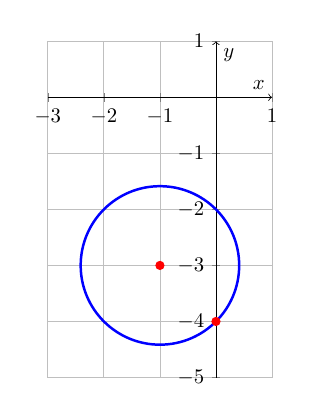
\begin{tikzpicture}[scale=.75]
				\begin{axis}[ 
					axis lines = middle,
					axis line style={->},
					ymin=-5, ymax=1,
					xmin=-3, xmax=1,
					xlabel={$x$},
					ylabel={$y$},
					axis equal image,
					grid=both,
					xtick distance=1,
					ytick distance=1
					]
					\addplot[red, mark=*, only marks] coordinates {(-1,-3) (0,-4)};
					\draw[color=blue,very thick] (axis cs:-1,-3) circle [radius=sqrt(2)];
				\end{axis}
			\end{tikzpicture}
	\item What is the center and the radius of a circle with equation $x^2+y^2+8x+14y+1=0$?
	\newpage
	\item Find the domain of the function.  Write your answer in interval and set builder notation.
		\begin{multicols}{2}\setlength{\columnseprule}{0.4pt}
			\begin{enumerate}
			\item $f(x)=\sqrt{3x-2}$\vskip 1in\mbox{}
			\item $g(x)=\dfrac{2x+1}{x^2-9}$\vskip 1in\mbox{}
		\end{enumerate}
		\end{multicols}
	\item For each function compute the given items then determine if the function is even/odd/neither.
		\begin{multicols}{2}\setlength{\columnseprule}{0.4pt}
			\begin{enumerate}
			\item $f(x)=3x^2-2$
				\begin{enumerate}\setlength{\itemsep}{2em}
					\item $f(0)$
					\item $f(4)$
					\item $f(-2)$
					\item $f(a)$
					\item $f(x+h)$
					\item $f(t^2+1)$
					\item $x$-intercepts
					\item $y$-intercepts
					\item the average value of $y=f(x)$ from $x=1$ to $x=3$\vskip 1in
					\item Is $f$ even/odd/both/neither?\vskip .75in\mbox{}
				\end{enumerate}
			\item $g(x)=2|x-1|-4$
				\begin{enumerate}\setlength{\itemsep}{2em}
					\item $g(0)$
					\item $g(4)$
					\item $g(-2)$
					\item $g(a)$
					\item $g(x+h)$
					\item $g(r^2+1)$
					\item $x$-intercepts
					\item $y$-intercepts
					\item the average value of $y=g(x)$ from $x=1$ to $x=3$\vskip 1in
					\item Is $g$ even/odd/both/neither?\vskip .75in\mbox{}
				\end{enumerate}
			%\item $f(x)=x^3-x$
		\end{enumerate}
		\end{multicols}
	\newpage
	\item Is the relation $\{(2,3),(-1,3),(5,3)\}$ a function? What is the domain of the relation? What is the range of the relation?\vskip 1in
	\item If $H(t)$ describes the height of a tree that is $t$ years old, then what does the average rate of change of $H$ from $t=1$ to $t=5$ represent? 
		\vskip 1in
	\item A company that makes thing-a-ma-bobs has a start up cost of \$16936. It costs the company \$1.54 to make each thing-a-ma-bob and the company charges \$4.27 for each thing-a-ma-bob. Let $x$	represent the number of thing-a-ma-bobs made.  
	\begin{enumerate}\setlength{\itemsep}{2em}
		\item Write a cost function for this company. 
		\item Write the revenue function for this company. 
		\item Write the profit function for this company. 
		\item What is the minimum number of thing-a-ma-bobs that the company must produce and sell to make a profit?\vskip 1in
	\end{enumerate}
	\item What does the graph of an even function look like? Sketch some examples.
		\vfill
	\item What does the graph of an odd function look like? Sketch some examples.
		\vfill
	\newpage
	\item Consider the graph of the function $h(x)$ on the left. The blank grid on the right is for you to possibly use in completing (d)-(f). (Up to you.)
		\begin{center}
			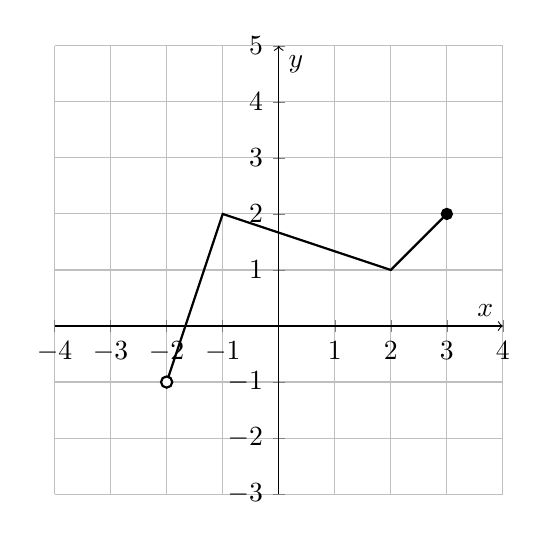
\begin{tikzpicture}%[scale=.75]
				\begin{axis}[ 
					axis lines = middle,
					axis line style={->},
					ymin=-3, ymax=5,
					xmin=-4, xmax=4,
					xlabel={$x$},
					ylabel={$y$},
					axis equal image,
					grid=both,
					xtick distance=1,
					ytick distance=1
					]
					\draw[-,thick] (-2,-1)-- (-1,2) -- (2,1) -- (3,2);
					%\draw (3.1,.75)   node[fill=white] {$y=h(x)$} ;
					\draw[fill=black] (axis cs:3,2) circle [radius=.1];
					\draw[fill=white,thick] (axis cs:-2,-1) circle [radius=.1];
				\end{axis}
			\end{tikzpicture}
			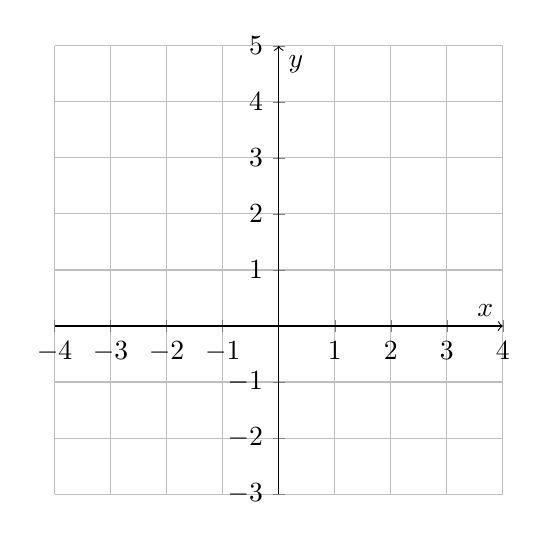
\begin{tikzpicture}%[scale=.75]
			\begin{axis}[ 
				axis lines = middle,
				axis line style={->},
				ymin=-3, ymax=5,
				xmin=-4, xmax=4,
				xlabel={$x$},
				ylabel={$y$},
				axis equal image,
				grid=both,
				xtick distance=1,
				ytick distance=1
				]
			\end{axis}
			\end{tikzpicture}
		\end{center}
		\begin{enumerate}
			\item Explain why the graph defines $y$ as a function of $x$.\vfill
			\item Determine $h(2)$.\vfill
			\item Determine $h(-1)$.\vfill
			\item Sketch a graph of $y=h(x-1)$. 
			\item Sketch a graph of $y=2h(x)$.
			\item Sketch a graph of $y=h(-x)$.
			\item What is the domain of $h(x)$?\vfill
			\item What is the range of $h(x)$?\vfill
			\item What are the $x-$ and $y-$intercepts of the graph?\vfill
			\item On what intervals is the function increasing?\vfill
			\item On what intervals is the function decreasing?\vfill
			\item Write $h(x)$ as a piecewise function by finding equations for each of the three linear portions of the graph.\vfill\vfill\vfill
		\end{enumerate}
	\newpage
	\item Given the piecwise function, evaluate the values.
		\[g(x)=\begin{cases}
			x+2&\text{if }x\leq -5\\
			|x+1|+2&\text{if }-5<x<0\\
			\frac{1}{3x+2}&\text{if }0\leq x\leq2\\
			x^2+x+1&\text{if }x>2\\
		\end{cases}\]
		\begin{multicols}{2}
			\begin{enumerate}\setlength{\itemsep}{2em}
			\item $f(0)$
			\item $f(-5)$
			\item $f(1)$
			\item $f(10)$
		\end{enumerate}
		\end{multicols}
		\vskip 1em
	\item Graph the piecewise function
		\[r(x)=\begin{cases}
			3x+2&\text{if } x\leq 1\\
			-5&\text{if }x>1
		\end{cases}\]
	\begin{center}
		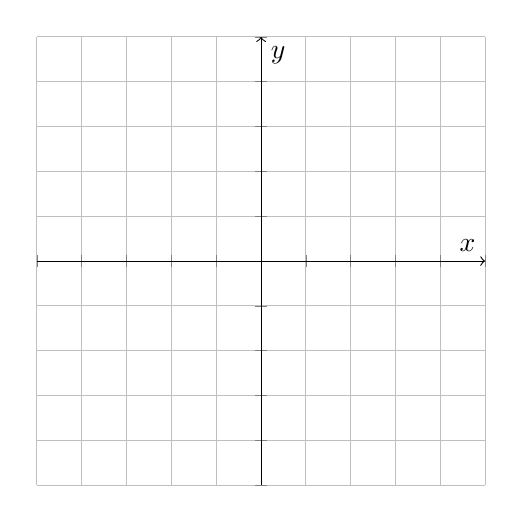
\begin{tikzpicture}%[scale=.75]
			\begin{axis}[ 
				axis lines = middle,
				axis line style={->},
				ymin=-10, ymax=10,
				xmin=-10, xmax=10,
				xlabel={$x$},
				ylabel={$y$},
				axis equal image,
				grid=both,
				xtick distance=2,
				ytick distance=2,
				xticklabels={},
				yticklabels={}
				]
			\end{axis}
		\end{tikzpicture}
	\end{center}
	\item Let $f(x)=x^2+1$, $g(x)=|x-2|$, $h(x)=4x-3$.
		\begin{enumerate}
			\item Compute $g(h(2))$.\vskip 2em
			\item Compute $f\circ g (-3)=f(g(-3))$.\vskip 2em
			\item Compute and simplify $f(h(x))$.\vfill
			\item Compute and simplify $h\circ h(x)=h(h(x))$.\vfill
		\end{enumerate}
	\newpage
	\item Given the graphs below
		\begin{center}
			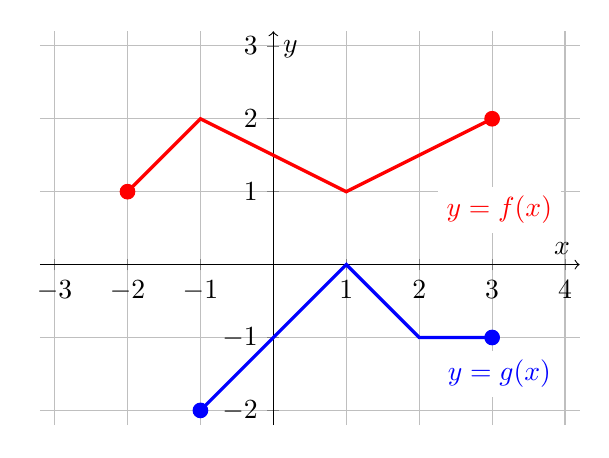
\begin{tikzpicture}
				\begin{axis}[ 
					axis lines = middle,
					axis line style={->},
					ymin=-2.2, ymax=3.2,
					xmin=-3.2, xmax=4.2,
					xlabel={$x$},
					ylabel={$y$},
					axis equal image,
					grid=both,
					xtick distance=1,
					ytick distance=1
					]
					\draw[-,very thick,red] (-2,1)-- (-1,2) -- (1,1) -- (3,2);
					\draw (3.1,.75)   node[red,fill=white] {$y=f(x)$} ;
					\draw[red,fill=red] (axis cs:3,2) circle [radius=.1];
					\draw[red,fill=red] (axis cs:-2,1) circle [radius=.1];
					\draw[-,very thick,blue] (-1,-2)-- (1,0) -- (2,-1) -- (3,-1);
					\draw (3.1,-1.5)   node[blue,fill=white] {$y=g(x)$} ;
					\draw[blue,fill=blue] (axis cs:3,-1) circle [radius=.1];
					\draw[fill=blue,blue] (axis cs:-1,-2) circle [radius=.1];
				\end{axis}
			\end{tikzpicture}
		\end{center}
		\begin{enumerate}\setlength{\itemsep}{4em}
			\item Compute $g(f(-2))$.
			\item Compute $f(g(2)))$.
			\item Compute $f\circ g(0))$.
			\item Compute $g\circ f(0))$.
			\item Compute $f\circ f(-1)$
		\end{enumerate}
		\vskip 3em
	\item Let  $H(x)=4(x-2)^{10}$. Which of the following pairs of functions $f(x)$ and $g(x)$ will produce $f\circ g(x)=H(x)$?  (There are two...) Can you find another decomposition?
		\begin{itemize}
			\item $f(x)=4x-2$ and $g(x)=x^{10}$
			\item $f(x)=x^{10}$ and $g(x)=4x-2$
			\item $f(x)=4x^{10}$ and $g(x)=x-2$
			\item $f(x)=x-2$ and $g(x)=4x^{10}$
			\item $f(x)=4x$ and $g(x)=(x-2)^{10}$
			\item $f(x)=(x-2)^{10}$ and $g(x)=4x$
		\end{itemize}
	\newpage
	
	\item For each Section in Chapter 2, write down the key terms and ideas.
	\begin{enumerate}
		\item Section 2.1: The Rectangular Coordinate System\vfill
		\item Section 2.2: Circles\vfill
		\item Section 2.3: Functions and Relations\vfill
		\item Section 2.4: Linear Equations in Two Variables and Linear Functions\vfill
		\newpage
		\item Section 2.5: Applications of Linear Equations and Modeling\vfill 
		\item Section 2.6: Transformations of Graphs\vfill 
		\item Section 2.7: Analyzing Graphs of Functions and Piecewise Defined Functions\vfill 
		\item Section 2.8: Algebra of Functions and Function Composition\vfill
	\end{enumerate}
\end{enumerate}
\end{document}